\subsection{Renyi divergenca normalnih porazdelitev}

Kot zgled si poglejmo izračun Renyi divergence za nekaj normalnih porazdelitev. Podajmo jih z enačbami:

\begin{equation}\label{norm_porazd}
	\begin{aligned}
		\N_1^{0,1}(x) &= \frac{1}{\sqrt{2\pi}}\cdot e^{-\frac{x^2}{2}} \\
		\N_2^{5,1}(x) &= \frac{1}{\sqrt{2\pi}}\cdot e^{-\frac{(x-5)^2}{2}} \\
		\N_3^{0,5}(x) &= \frac{1}{5\sqrt{2\pi}}\cdot e^{-\frac{x^2}{50}} \\
		\N_4^{0,10}(x) &= \frac{1}{10\sqrt{2\pi}}\cdot e^{-\frac{x^2}{200}}.
	\end{aligned}
\end{equation}

kjer je $\N_i^{\mu_i, \sigma_i}$ gostota verjetnosti porazdelitve $P_i$. Za predstavo si oglejmo še grafe teh verjetnostnih porazdelitev:

\begin{figure}[!ht]
	\centering
	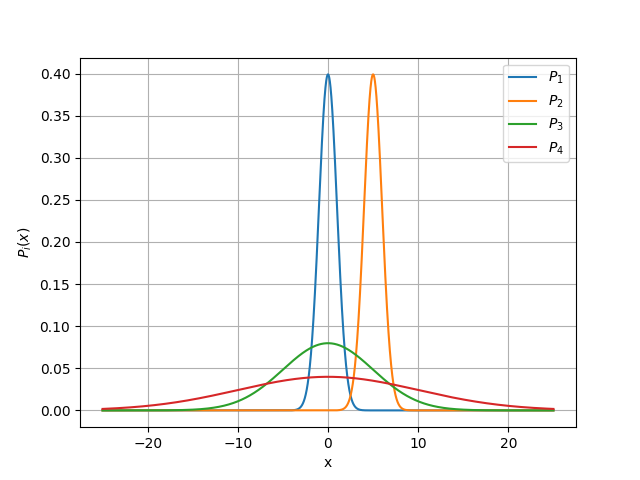
\includegraphics[scale=0.8]{normalne4}
	\caption{Normalne porazdelitve.}
\end{figure}

Brez simbolnega računanja si poglejmo divergenco med normalnimi porazdelitvami \eqref{norm_porazd}.

\begin{figure}[!ht]
	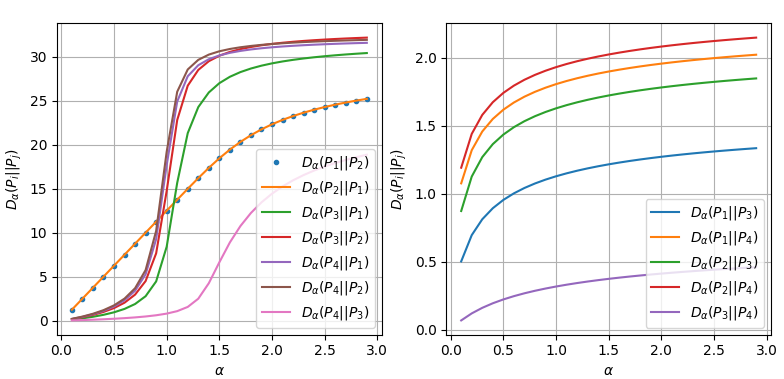
\includegraphics[scale=0.8]{divnorm}
	\caption{Divergence normalnih porazdelitev.}
	\label{divergence}
\end{figure}
\pagebreak
Na podlagi izračunov omenimo ugotovitvi:
\begin{enumerate}
	\item Opazimo, da bo vrednost Renyi divergence zelo velika, če bo varianca prve porazdelitve večja kot varianca druge porazdelitve in majhna, če bo varianca prve porazdelitve manjša kot varianca druge porazdelitve.
	\item Če je varianca porazdelitev $P_1$ in $P_2$ enaka, je Renyi divergenca simetrična, t.j. 
	\begin{equation*}
		D(P_1 \| P_2) = D^{\ast}(P_1 \| P_2) = D(P_2 \| P_1).
	\end{equation*}
\end{enumerate}

Če lahko sklepamo na podlagi Renyi divergence normalnih porazdelitev smo ugotovili, da na Renyi divergenco zelo vpliva razmerje med variancama prve in druge porazdelitve. Zaradi tega je lahko razlika med vrednostjo Renyi divergence in vrednostjo dualne Renyi divergence zelo velika.

Brez dokaza omenimo še, da translacija sistema ne vpliva na izračun Renyi divergence normalnih porazdelitev, to pomeni:
\begin{equation}
	D_\alpha\Big(\N^{\mu_1, \sigma_1}(x) \| \N^{\mu_2, \sigma_2}(x)\Big) = D_\alpha\Big(\N^{\mu_1, \sigma_1}(x - a) \| \N^{\mu_2, \sigma_2}(x - a)\Big),
\end{equation}
kjer je $a \in \mathbb{R}$.

\begin{opomba}
	Izračun divergenc in izris grafov sta bila narejena s programskim jezikom \texttt{Python3}.
\end{opomba}